% Created by tikzDevice version 0.12 on 2019-05-15 08:29:24
% !TEX encoding = UTF-8 Unicode
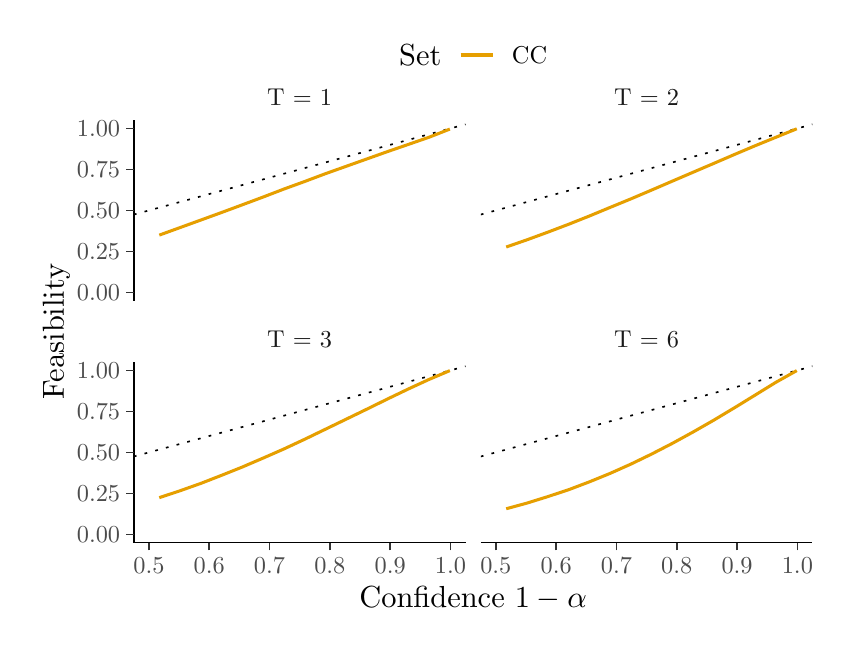
\begin{tikzpicture}[x=1pt,y=1pt]
\definecolor{fillColor}{RGB}{255,255,255}
\path[use as bounding box,fill=fillColor,fill opacity=0.00] (0,0) rectangle (289.08,216.81);
\begin{scope}
\path[clip] (  0.00,  0.00) rectangle (289.08,216.81);
\definecolor{drawColor}{RGB}{255,255,255}
\definecolor{fillColor}{RGB}{255,255,255}

\path[draw=drawColor,line width= 0.6pt,line join=round,line cap=round,fill=fillColor] (  0.00,  0.00) rectangle (289.08,216.81);
\end{scope}
\begin{scope}
\path[clip] ( 38.36,118.15) rectangle (158.22,183.28);
\definecolor{fillColor}{RGB}{255,255,255}

\path[fill=fillColor] ( 38.36,118.15) rectangle (158.22,183.28);
\definecolor{drawColor}{RGB}{0,0,0}

\path[draw=drawColor,line width= 0.6pt,dash pattern=on 1pt off 3pt ,line join=round] ( 38.36,149.28) -- (158.22,181.88);
\definecolor{drawColor}{RGB}{230,159,0}

\path[draw=drawColor,line width= 1.1pt,line join=round] ( 47.56,141.85) --
	( 55.06,144.57) --
	( 62.56,147.29) --
	( 70.06,150.02) --
	( 77.56,152.80) --
	( 85.06,155.60) --
	( 92.56,158.48) --
	(100.06,161.21) --
	(107.56,164.03) --
	(115.06,166.70) --
	(122.56,169.37) --
	(130.06,172.04) --
	(137.55,174.62) --
	(145.05,177.22) --
	(152.55,180.16);
\end{scope}
\begin{scope}
\path[clip] ( 38.36, 30.72) rectangle (158.22, 95.85);
\definecolor{fillColor}{RGB}{255,255,255}

\path[fill=fillColor] ( 38.36, 30.72) rectangle (158.22, 95.85);
\definecolor{drawColor}{RGB}{0,0,0}

\path[draw=drawColor,line width= 0.6pt,dash pattern=on 1pt off 3pt ,line join=round] ( 38.36, 61.85) -- (158.22, 94.46);
\definecolor{drawColor}{RGB}{230,159,0}

\path[draw=drawColor,line width= 1.1pt,line join=round] ( 47.56, 46.98) --
	( 55.06, 49.47) --
	( 62.56, 52.13) --
	( 70.06, 55.05) --
	( 77.56, 58.05) --
	( 85.06, 61.27) --
	( 92.56, 64.56) --
	(100.06, 68.06) --
	(107.56, 71.69) --
	(115.06, 75.32) --
	(122.56, 78.96) --
	(130.06, 82.65) --
	(137.55, 86.25) --
	(145.05, 89.71) --
	(152.55, 92.88);
\end{scope}
\begin{scope}
\path[clip] (163.72,118.15) rectangle (283.58,183.28);
\definecolor{fillColor}{RGB}{255,255,255}

\path[fill=fillColor] (163.72,118.15) rectangle (283.58,183.28);
\definecolor{drawColor}{RGB}{0,0,0}

\path[draw=drawColor,line width= 0.6pt,dash pattern=on 1pt off 3pt ,line join=round] (163.72,149.28) -- (283.58,181.88);
\definecolor{drawColor}{RGB}{230,159,0}

\path[draw=drawColor,line width= 1.1pt,line join=round] (172.92,137.55) --
	(180.42,140.15) --
	(187.92,142.90) --
	(195.42,145.75) --
	(202.92,148.73) --
	(210.42,151.84) --
	(217.92,154.92) --
	(225.42,158.11) --
	(232.92,161.34) --
	(240.42,164.56) --
	(247.92,167.76) --
	(255.41,170.99) --
	(262.91,174.16) --
	(270.41,177.22) --
	(277.91,180.27);
\end{scope}
\begin{scope}
\path[clip] (163.72, 30.72) rectangle (283.58, 95.85);
\definecolor{fillColor}{RGB}{255,255,255}

\path[fill=fillColor] (163.72, 30.72) rectangle (283.58, 95.85);
\definecolor{drawColor}{RGB}{0,0,0}

\path[draw=drawColor,line width= 0.6pt,dash pattern=on 1pt off 3pt ,line join=round] (163.72, 61.85) -- (283.58, 94.46);
\definecolor{drawColor}{RGB}{230,159,0}

\path[draw=drawColor,line width= 1.1pt,line join=round] (172.92, 42.97) --
	(180.42, 45.01) --
	(187.92, 47.35) --
	(195.42, 49.83) --
	(202.92, 52.67) --
	(210.42, 55.73) --
	(217.92, 59.08) --
	(225.42, 62.71) --
	(232.92, 66.58) --
	(240.42, 70.69) --
	(247.92, 74.98) --
	(255.41, 79.46) --
	(262.91, 84.07) --
	(270.41, 88.69) --
	(277.91, 92.89);
\end{scope}
\begin{scope}
\path[clip] ( 38.36, 95.85) rectangle (158.22,112.65);
\definecolor{drawColor}{RGB}{255,255,255}
\definecolor{fillColor}{RGB}{255,255,255}

\path[draw=drawColor,line width= 1.1pt,line join=round,line cap=round,fill=fillColor] ( 38.36, 95.85) rectangle (158.22,112.65);
\definecolor{drawColor}{gray}{0.10}

\node[text=drawColor,anchor=base,inner sep=0pt, outer sep=0pt, scale=  0.88] at ( 98.29,101.22) {T = 3};
\end{scope}
\begin{scope}
\path[clip] (163.72, 95.85) rectangle (283.58,112.65);
\definecolor{drawColor}{RGB}{255,255,255}
\definecolor{fillColor}{RGB}{255,255,255}

\path[draw=drawColor,line width= 1.1pt,line join=round,line cap=round,fill=fillColor] (163.72, 95.85) rectangle (283.58,112.65);
\definecolor{drawColor}{gray}{0.10}

\node[text=drawColor,anchor=base,inner sep=0pt, outer sep=0pt, scale=  0.88] at (223.65,101.22) {T = 6};
\end{scope}
\begin{scope}
\path[clip] ( 38.36,183.28) rectangle (158.22,200.08);
\definecolor{drawColor}{RGB}{255,255,255}
\definecolor{fillColor}{RGB}{255,255,255}

\path[draw=drawColor,line width= 1.1pt,line join=round,line cap=round,fill=fillColor] ( 38.36,183.28) rectangle (158.22,200.08);
\definecolor{drawColor}{gray}{0.10}

\node[text=drawColor,anchor=base,inner sep=0pt, outer sep=0pt, scale=  0.88] at ( 98.29,188.65) {T = 1};
\end{scope}
\begin{scope}
\path[clip] (163.72,183.28) rectangle (283.58,200.08);
\definecolor{drawColor}{RGB}{255,255,255}
\definecolor{fillColor}{RGB}{255,255,255}

\path[draw=drawColor,line width= 1.1pt,line join=round,line cap=round,fill=fillColor] (163.72,183.28) rectangle (283.58,200.08);
\definecolor{drawColor}{gray}{0.10}

\node[text=drawColor,anchor=base,inner sep=0pt, outer sep=0pt, scale=  0.88] at (223.65,188.65) {T = 2};
\end{scope}
\begin{scope}
\path[clip] (  0.00,  0.00) rectangle (289.08,216.81);
\definecolor{drawColor}{RGB}{0,0,0}

\path[draw=drawColor,line width= 0.6pt,line join=round] ( 38.36, 30.72) --
	(158.22, 30.72);
\end{scope}
\begin{scope}
\path[clip] (  0.00,  0.00) rectangle (289.08,216.81);
\definecolor{drawColor}{gray}{0.20}

\path[draw=drawColor,line width= 0.6pt,line join=round] ( 43.81, 27.97) --
	( 43.81, 30.72);

\path[draw=drawColor,line width= 0.6pt,line join=round] ( 65.60, 27.97) --
	( 65.60, 30.72);

\path[draw=drawColor,line width= 0.6pt,line join=round] ( 87.39, 27.97) --
	( 87.39, 30.72);

\path[draw=drawColor,line width= 0.6pt,line join=round] (109.19, 27.97) --
	(109.19, 30.72);

\path[draw=drawColor,line width= 0.6pt,line join=round] (130.98, 27.97) --
	(130.98, 30.72);

\path[draw=drawColor,line width= 0.6pt,line join=round] (152.77, 27.97) --
	(152.77, 30.72);
\end{scope}
\begin{scope}
\path[clip] (  0.00,  0.00) rectangle (289.08,216.81);
\definecolor{drawColor}{gray}{0.30}

\node[text=drawColor,anchor=base,inner sep=0pt, outer sep=0pt, scale=  0.88] at ( 43.81, 19.71) {0.5};

\node[text=drawColor,anchor=base,inner sep=0pt, outer sep=0pt, scale=  0.88] at ( 65.60, 19.71) {0.6};

\node[text=drawColor,anchor=base,inner sep=0pt, outer sep=0pt, scale=  0.88] at ( 87.39, 19.71) {0.7};

\node[text=drawColor,anchor=base,inner sep=0pt, outer sep=0pt, scale=  0.88] at (109.19, 19.71) {0.8};

\node[text=drawColor,anchor=base,inner sep=0pt, outer sep=0pt, scale=  0.88] at (130.98, 19.71) {0.9};

\node[text=drawColor,anchor=base,inner sep=0pt, outer sep=0pt, scale=  0.88] at (152.77, 19.71) {1.0};
\end{scope}
\begin{scope}
\path[clip] (  0.00,  0.00) rectangle (289.08,216.81);
\definecolor{drawColor}{RGB}{0,0,0}

\path[draw=drawColor,line width= 0.6pt,line join=round] (163.72, 30.72) --
	(283.58, 30.72);
\end{scope}
\begin{scope}
\path[clip] (  0.00,  0.00) rectangle (289.08,216.81);
\definecolor{drawColor}{gray}{0.20}

\path[draw=drawColor,line width= 0.6pt,line join=round] (169.17, 27.97) --
	(169.17, 30.72);

\path[draw=drawColor,line width= 0.6pt,line join=round] (190.96, 27.97) --
	(190.96, 30.72);

\path[draw=drawColor,line width= 0.6pt,line join=round] (212.75, 27.97) --
	(212.75, 30.72);

\path[draw=drawColor,line width= 0.6pt,line join=round] (234.55, 27.97) --
	(234.55, 30.72);

\path[draw=drawColor,line width= 0.6pt,line join=round] (256.34, 27.97) --
	(256.34, 30.72);

\path[draw=drawColor,line width= 0.6pt,line join=round] (278.13, 27.97) --
	(278.13, 30.72);
\end{scope}
\begin{scope}
\path[clip] (  0.00,  0.00) rectangle (289.08,216.81);
\definecolor{drawColor}{gray}{0.30}

\node[text=drawColor,anchor=base,inner sep=0pt, outer sep=0pt, scale=  0.88] at (169.17, 19.71) {0.5};

\node[text=drawColor,anchor=base,inner sep=0pt, outer sep=0pt, scale=  0.88] at (190.96, 19.71) {0.6};

\node[text=drawColor,anchor=base,inner sep=0pt, outer sep=0pt, scale=  0.88] at (212.75, 19.71) {0.7};

\node[text=drawColor,anchor=base,inner sep=0pt, outer sep=0pt, scale=  0.88] at (234.55, 19.71) {0.8};

\node[text=drawColor,anchor=base,inner sep=0pt, outer sep=0pt, scale=  0.88] at (256.34, 19.71) {0.9};

\node[text=drawColor,anchor=base,inner sep=0pt, outer sep=0pt, scale=  0.88] at (278.13, 19.71) {1.0};
\end{scope}
\begin{scope}
\path[clip] (  0.00,  0.00) rectangle (289.08,216.81);
\definecolor{drawColor}{RGB}{0,0,0}

\path[draw=drawColor,line width= 0.6pt,line join=round] ( 38.36,118.15) --
	( 38.36,183.28);
\end{scope}
\begin{scope}
\path[clip] (  0.00,  0.00) rectangle (289.08,216.81);
\definecolor{drawColor}{gray}{0.30}

\node[text=drawColor,anchor=base east,inner sep=0pt, outer sep=0pt, scale=  0.88] at ( 33.41,118.08) {0.00};

\node[text=drawColor,anchor=base east,inner sep=0pt, outer sep=0pt, scale=  0.88] at ( 33.41,132.91) {0.25};

\node[text=drawColor,anchor=base east,inner sep=0pt, outer sep=0pt, scale=  0.88] at ( 33.41,147.73) {0.50};

\node[text=drawColor,anchor=base east,inner sep=0pt, outer sep=0pt, scale=  0.88] at ( 33.41,162.55) {0.75};

\node[text=drawColor,anchor=base east,inner sep=0pt, outer sep=0pt, scale=  0.88] at ( 33.41,177.37) {1.00};
\end{scope}
\begin{scope}
\path[clip] (  0.00,  0.00) rectangle (289.08,216.81);
\definecolor{drawColor}{gray}{0.20}

\path[draw=drawColor,line width= 0.6pt,line join=round] ( 35.61,121.11) --
	( 38.36,121.11);

\path[draw=drawColor,line width= 0.6pt,line join=round] ( 35.61,135.94) --
	( 38.36,135.94);

\path[draw=drawColor,line width= 0.6pt,line join=round] ( 35.61,150.76) --
	( 38.36,150.76);

\path[draw=drawColor,line width= 0.6pt,line join=round] ( 35.61,165.58) --
	( 38.36,165.58);

\path[draw=drawColor,line width= 0.6pt,line join=round] ( 35.61,180.40) --
	( 38.36,180.40);
\end{scope}
\begin{scope}
\path[clip] (  0.00,  0.00) rectangle (289.08,216.81);
\definecolor{drawColor}{RGB}{0,0,0}

\path[draw=drawColor,line width= 0.6pt,line join=round] ( 38.36, 30.72) --
	( 38.36, 95.85);
\end{scope}
\begin{scope}
\path[clip] (  0.00,  0.00) rectangle (289.08,216.81);
\definecolor{drawColor}{gray}{0.30}

\node[text=drawColor,anchor=base east,inner sep=0pt, outer sep=0pt, scale=  0.88] at ( 33.41, 30.65) {0.00};

\node[text=drawColor,anchor=base east,inner sep=0pt, outer sep=0pt, scale=  0.88] at ( 33.41, 45.48) {0.25};

\node[text=drawColor,anchor=base east,inner sep=0pt, outer sep=0pt, scale=  0.88] at ( 33.41, 60.30) {0.50};

\node[text=drawColor,anchor=base east,inner sep=0pt, outer sep=0pt, scale=  0.88] at ( 33.41, 75.12) {0.75};

\node[text=drawColor,anchor=base east,inner sep=0pt, outer sep=0pt, scale=  0.88] at ( 33.41, 89.94) {1.00};
\end{scope}
\begin{scope}
\path[clip] (  0.00,  0.00) rectangle (289.08,216.81);
\definecolor{drawColor}{gray}{0.20}

\path[draw=drawColor,line width= 0.6pt,line join=round] ( 35.61, 33.68) --
	( 38.36, 33.68);

\path[draw=drawColor,line width= 0.6pt,line join=round] ( 35.61, 48.51) --
	( 38.36, 48.51);

\path[draw=drawColor,line width= 0.6pt,line join=round] ( 35.61, 63.33) --
	( 38.36, 63.33);

\path[draw=drawColor,line width= 0.6pt,line join=round] ( 35.61, 78.15) --
	( 38.36, 78.15);

\path[draw=drawColor,line width= 0.6pt,line join=round] ( 35.61, 92.97) --
	( 38.36, 92.97);
\end{scope}
\begin{scope}
\path[clip] (  0.00,  0.00) rectangle (289.08,216.81);
\definecolor{drawColor}{RGB}{0,0,0}

\node[text=drawColor,anchor=base,inner sep=0pt, outer sep=0pt, scale=  1.10] at (160.97,  7.44) {Confidence $1 - \alpha$};
\end{scope}
\begin{scope}
\path[clip] (  0.00,  0.00) rectangle (289.08,216.81);
\definecolor{drawColor}{RGB}{0,0,0}

\node[text=drawColor,rotate= 90.00,anchor=base,inner sep=0pt, outer sep=0pt, scale=  1.10] at ( 13.08,107.00) {Feasibility};
\end{scope}
\begin{scope}
\path[clip] (  0.00,  0.00) rectangle (289.08,216.81);
\definecolor{fillColor}{RGB}{255,255,255}

\path[fill=fillColor] (134.25,211.08) rectangle (187.69,211.31);
\end{scope}
\begin{scope}
\path[clip] (  0.00,  0.00) rectangle (289.08,216.81);
\definecolor{drawColor}{RGB}{0,0,0}

\node[text=drawColor,anchor=base west,inner sep=0pt, outer sep=0pt, scale=  1.10] at (134.25,203.14) {Set};
\end{scope}
\begin{scope}
\path[clip] (  0.00,  0.00) rectangle (289.08,216.81);
\definecolor{drawColor}{RGB}{230,159,0}

\path[draw=drawColor,line width= 1.1pt,line join=round] (156.47,206.93) -- (168.03,206.93);
\end{scope}
\begin{scope}
\path[clip] (  0.00,  0.00) rectangle (289.08,216.81);
\definecolor{drawColor}{RGB}{0,0,0}

\node[text=drawColor,anchor=base west,inner sep=0pt, outer sep=0pt, scale=  0.88] at (174.98,203.90) {CC};
\end{scope}
\end{tikzpicture}
